\section{Prediction for unassociated sources in 3FGL and comparison with 4FGL}
\lb{sec:3FGLprediction}




Comment: Create a table with sources which are more likely to be pulsars (select about 20 the most likely candidates).
Compare the accuracy of the algorithm for the sources which have an associate now in the 4FGL catalog.\\

In this section we use the best algorithms from the previous section to predict classes for the unassociated sources in the 3FGL. We then use the associations which exist for some of these sources in the 4FGL to check the accuracy of our methods on the unassociated data. In this section we work only with Random Forests, Neural Networks, AdaBoost, and Logistic Regression. \\


\subsection{3FGL Unassociated sources with Association in 4FGL}
There were a total of 286 sources without associations in 3FGL but which had a corresponding assocation in 4FGL. We trained our algorithms on the entire associated data from the 3FGL, and then used tested our algorithms on these 286 sources. The probabilistic version is discussed in the next section.  \\

The following were the optimized results we obtained for this case:\\

\begin{table}[!h]
    \tiny
    \centering
    \renewcommand{\tabcolsep}{1mm}
\renewcommand{\arraystretch}{1.5}

    \begin{tabular}{|c|c|c|}
    \hline
    Algorithm Name&Parameters & Accuracy\\
    \hline
    Random Forest& 50 trees and 12 max depth & 96.22   \\
    \hline
    Neural Network & 200 epochs, 20 neurons, tanh     &  95.97 \\
    \hline %\midrule   -> aakash do you mean this?
    Gradient Boost& 20,5    &   95.8  \\
    \hline %\midrule   -> aakash do you mean this?
    Logistic Regression& all solvers &to put  \\
    \hline
     
    \end{tabular}

    \caption{Testing Accuracy of 4 algorithms on 3FGL unassociated data}
    \label{tab:my_labe2l}
\end{table}


As can be seen above, the best accuracies were found with less complicated models, which allowed bias to be low. The models were complicated enough to neither under, nor overtrain. \\

\subsection{3FGL Probabilistic classification} 

\begin{figure}[h]
%\centerin
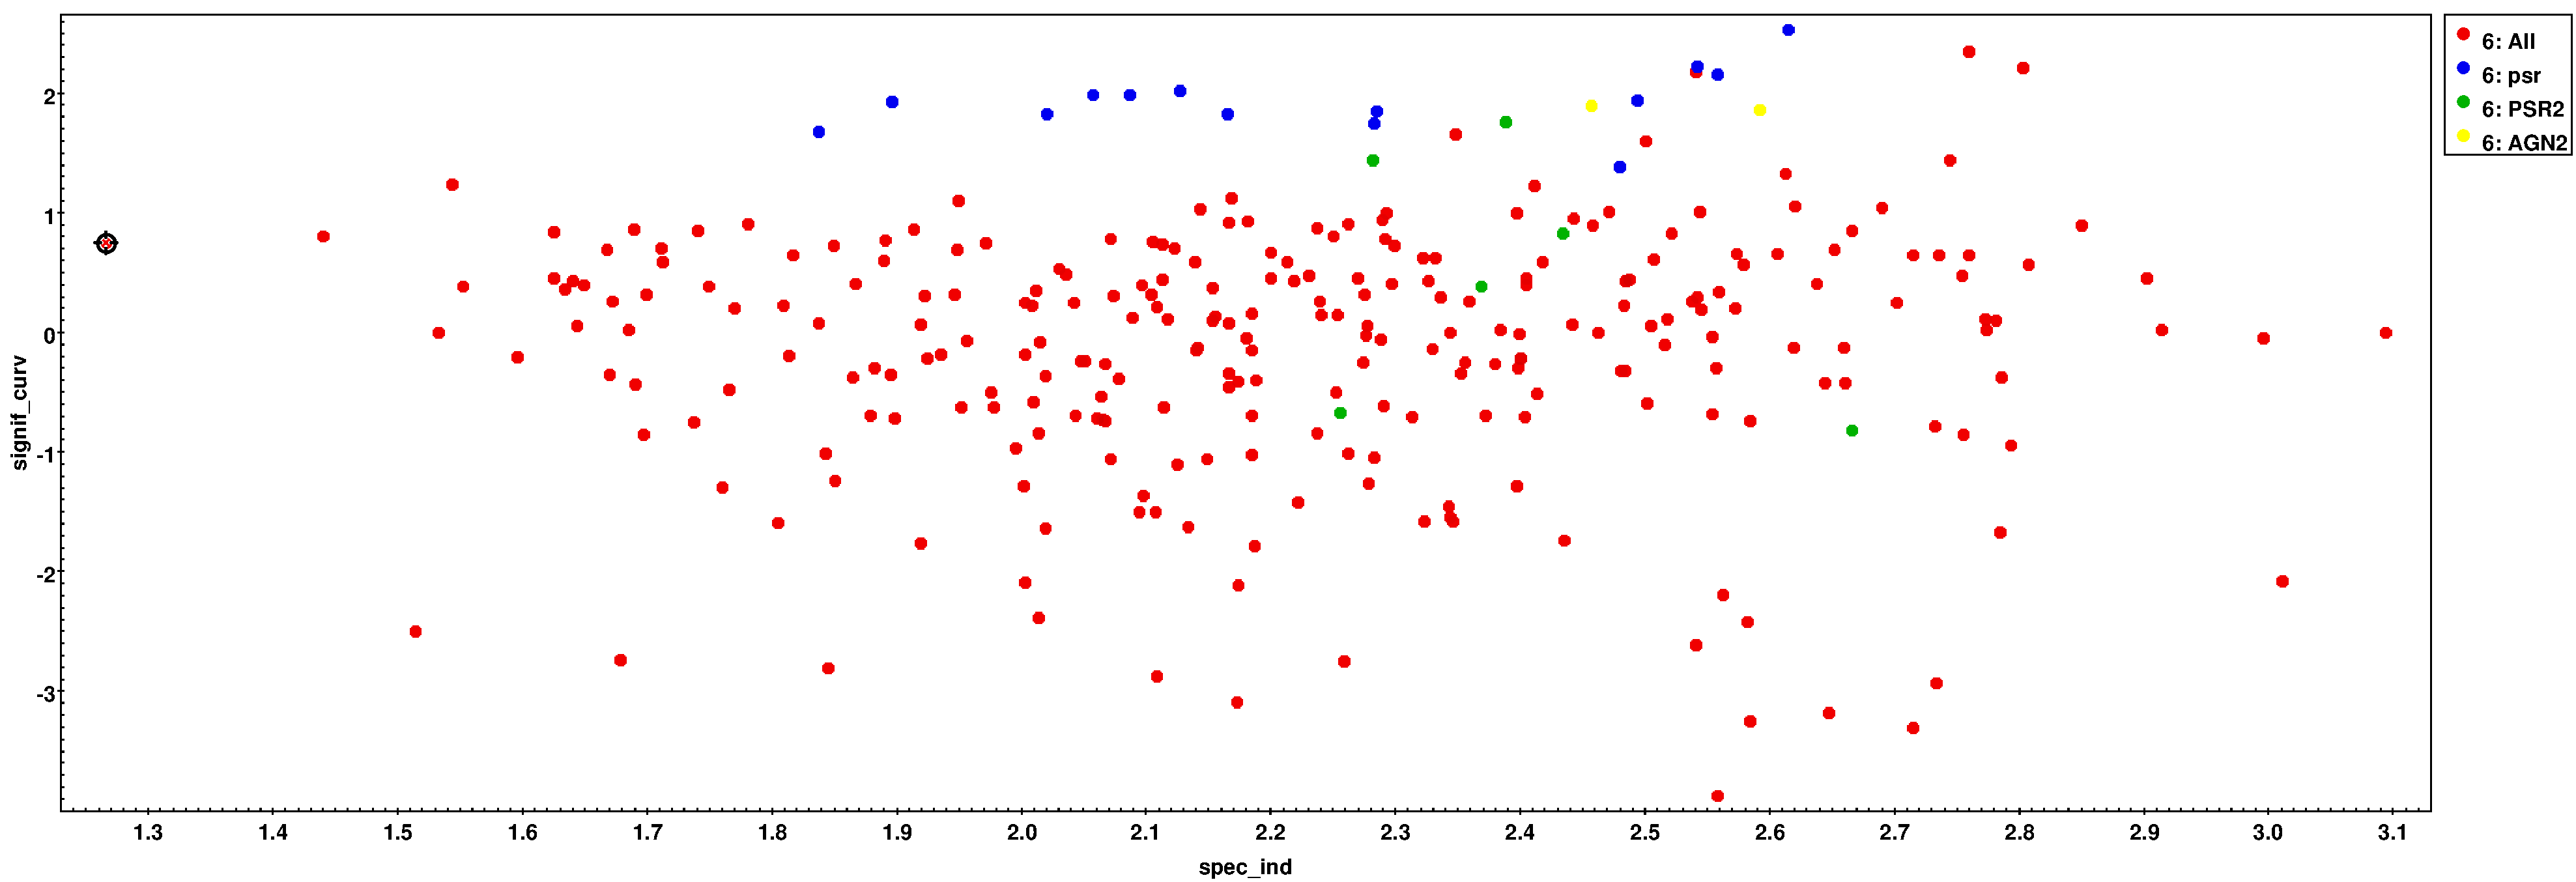
\includegraphics[width=\twopicsp\textwidth]{plots/cat_allalgos_outliers_PSR_AGN.pdf}
\caption{A comparison of the outliers in the test predictions}
\label{fig:Maps_data}
\end{figure}
